%%%%%% Taken from Fall 2015 Midterm 2e %%%%%%
%%%%%% Can also be found at /exam/src/fa15/mt2e/env.tex %%%%%%

\question Draw the box and pointer diagram that results from executing the
code below until the entire program is finished or an error occurs:

\begin{lstlisting}
w = [2, 2]
z = [2, 2, w]
x = z[w[0]]
y = list(x)
x.append([w.pop()])
y, x = z[2], y
w[0] = z.pop()
\end{lstlisting}

\begin{solution}[0.5in]
\begin{center}
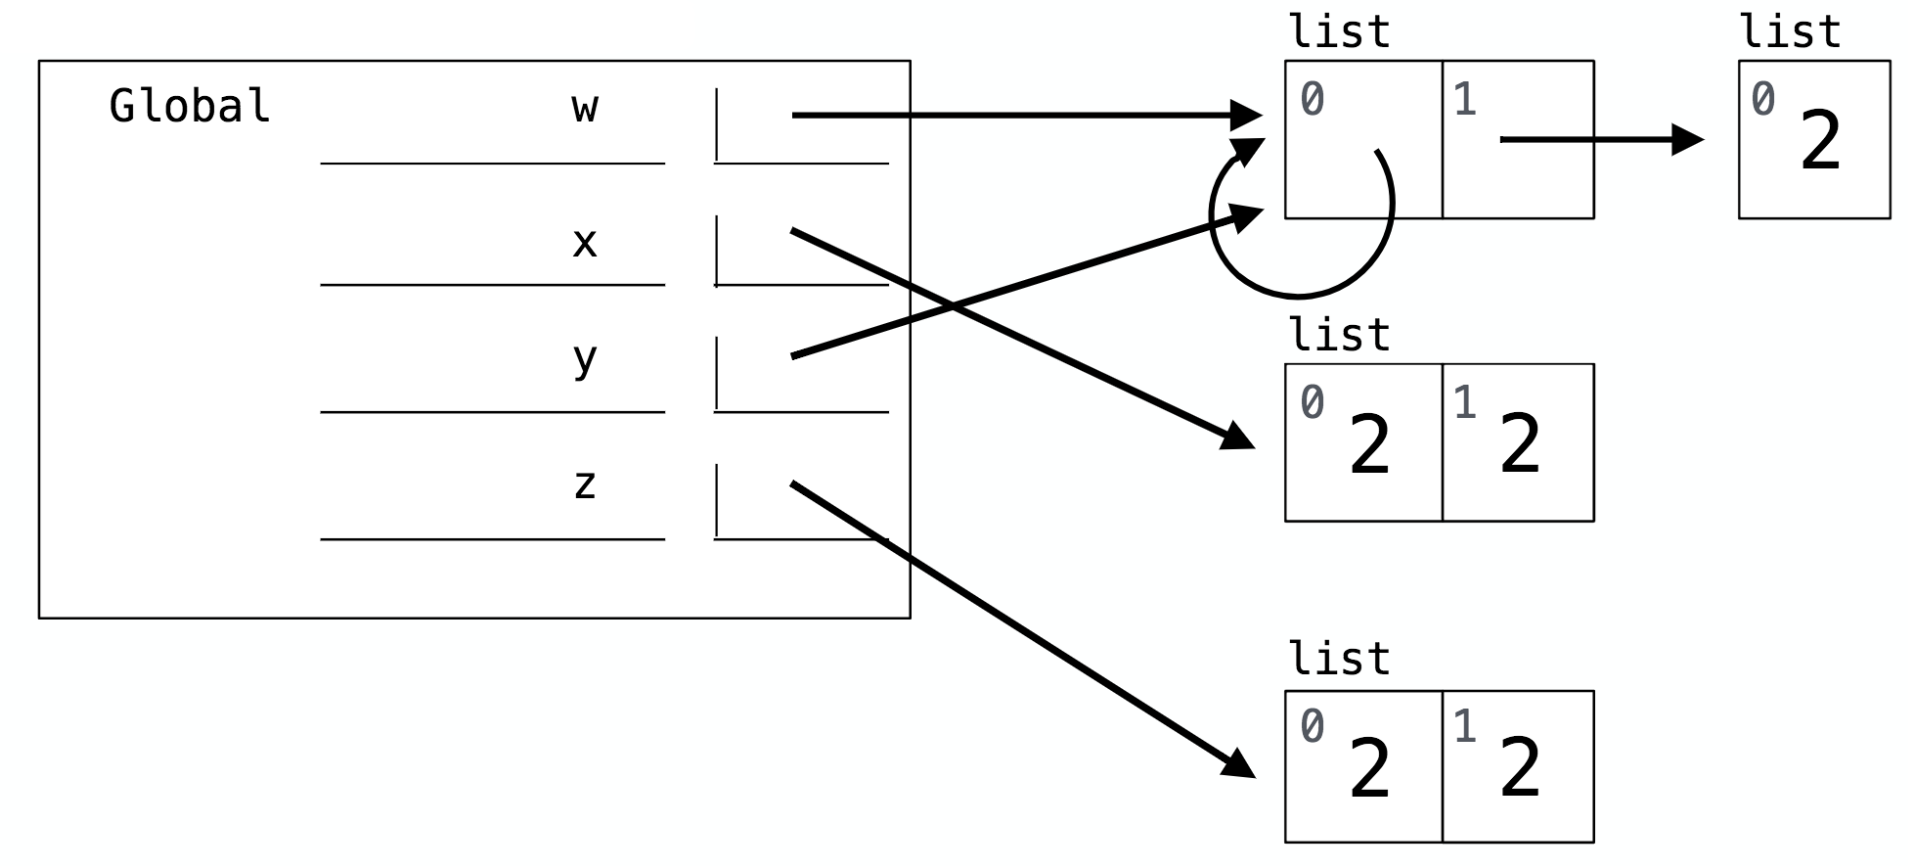
\includegraphics[scale=.4]{abcdsol.png}
\end{center}
\end{solution}
